% !TEX encoding = UTF-8
% !TEX program = pdflatex
% !TEX root = presentazione.tex
% !TeX spellcheck = it_IT
%
\begin{frame}[t]{Tariffe - Confronti}
	\begin{figure}[h]
	\centering
	    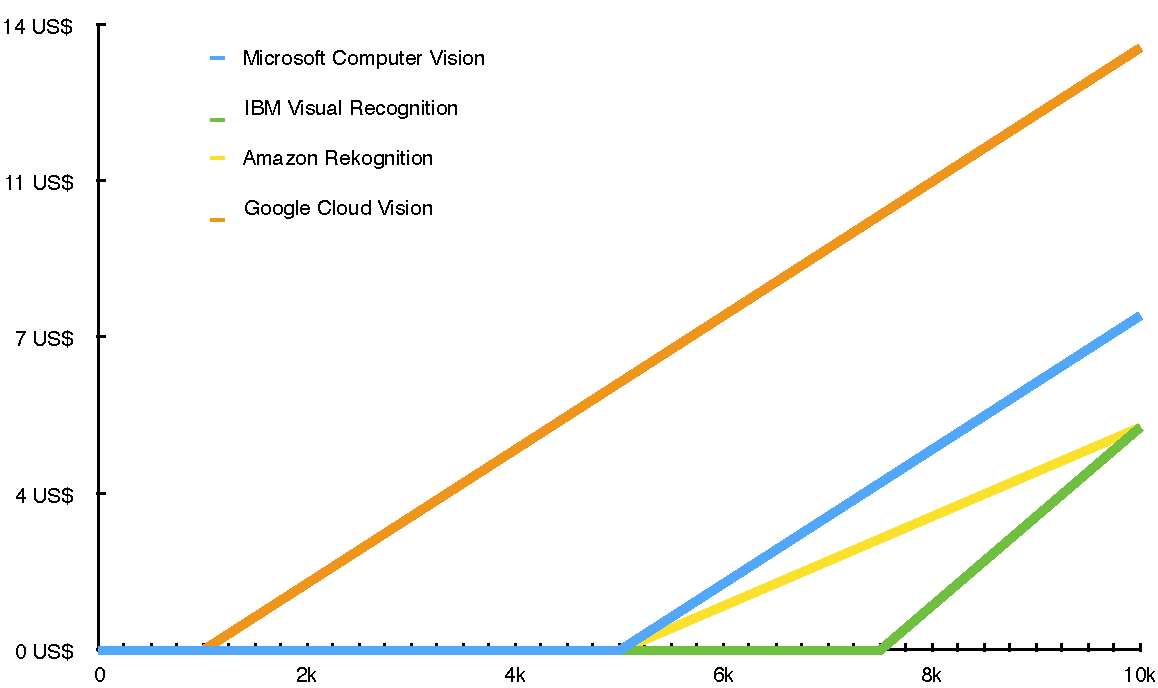
\includegraphics[width=.6\paperwidth,keepaspectratio=true]{../../doc/img/grafico1}
		{\tiny \caption{Riconoscimento oggetti con piano gratuito (da 0 a 10K immagini).}}
		\label{fig:tariffe-riconoscimento-oggetti-con-gratuito}
	\end{figure}
\end{frame}
%
%----------------------------------------------------------------------------------------
%	APPUNTI:
% 		- ricordarsi che ibm ne ha di più ma fa il conteggio giornaliero
%		- contiamo 1 chiamata - 1 immagine così viene più semplice
%----------------------------------------------------------------------------------------
